\documentclass[12pt]{article}
\usepackage[paperwidth=54cm,paperheight=36cm,margin=0.8cm]{geometry}
\usepackage{tikz}
\usetikzlibrary{arrows.meta, fit, calc, backgrounds, positioning}
\usepackage{xcolor}
\pagestyle{empty}

%% ── Palette ──────────────────────────────────────────────────────────────────
\definecolor{bg}    {HTML}{0D1117}   % page background
\definecolor{panel} {HTML}{161B22}   % dark panel (for color blending)
\definecolor{cIn}   {HTML}{0EA5E9}   % sky-500
\definecolor{cPerc} {HTML}{7C3AED}   % violet-700
\definecolor{cEng}  {HTML}{D97706}   % amber-600
\definecolor{cAI}   {HTML}{059669}   % emerald-600
\definecolor{cOut}  {HTML}{DC2626}   % red-600
\definecolor{cUI}   {HTML}{DB2777}   % pink-600
\definecolor{cArr}  {HTML}{64748B}
\definecolor{cTxt}  {HTML}{F8FAFC}
\definecolor{cSub}  {HTML}{94A3B8}
\definecolor{cHead} {HTML}{E2E8F0}

%% ── Styles ───────────────────────────────────────────────────────────────────
\tikzset{
  %--- node box: dark fill (color blended with panel) + bright text
  nd/.style 2 args={
    draw=#1, fill=#1!45!panel,
    rounded corners=5pt,
    text=cTxt, minimum width=#2, minimum height=0.9cm,
    align=center, inner sep=7pt,
    font=\sffamily\large\bfseries, line width=1.5pt
  },
  %--- sub-label
  sl/.style={text=cSub, font=\sffamily\small, align=center},
  %--- layer frame
  lyr/.style={
    draw=#1!80, fill=#1!12!bg,
    rounded corners=9pt, line width=2pt, inner sep=15pt
  },
  %--- solid arrow
  ar/.style={
    -{Stealth[length=8pt,width=6pt]},
    line width=1.7pt, color=cArr,
    shorten >=2pt, shorten <=2pt
  },
  %--- dashed arrow
  ard/.style={ar, dashed},
  %--- edge label
  el/.style={font=\sffamily\scriptsize\bfseries, text=cHead,
             fill=bg, inner sep=3pt},
}

\begin{document}
\pagecolor{bg}
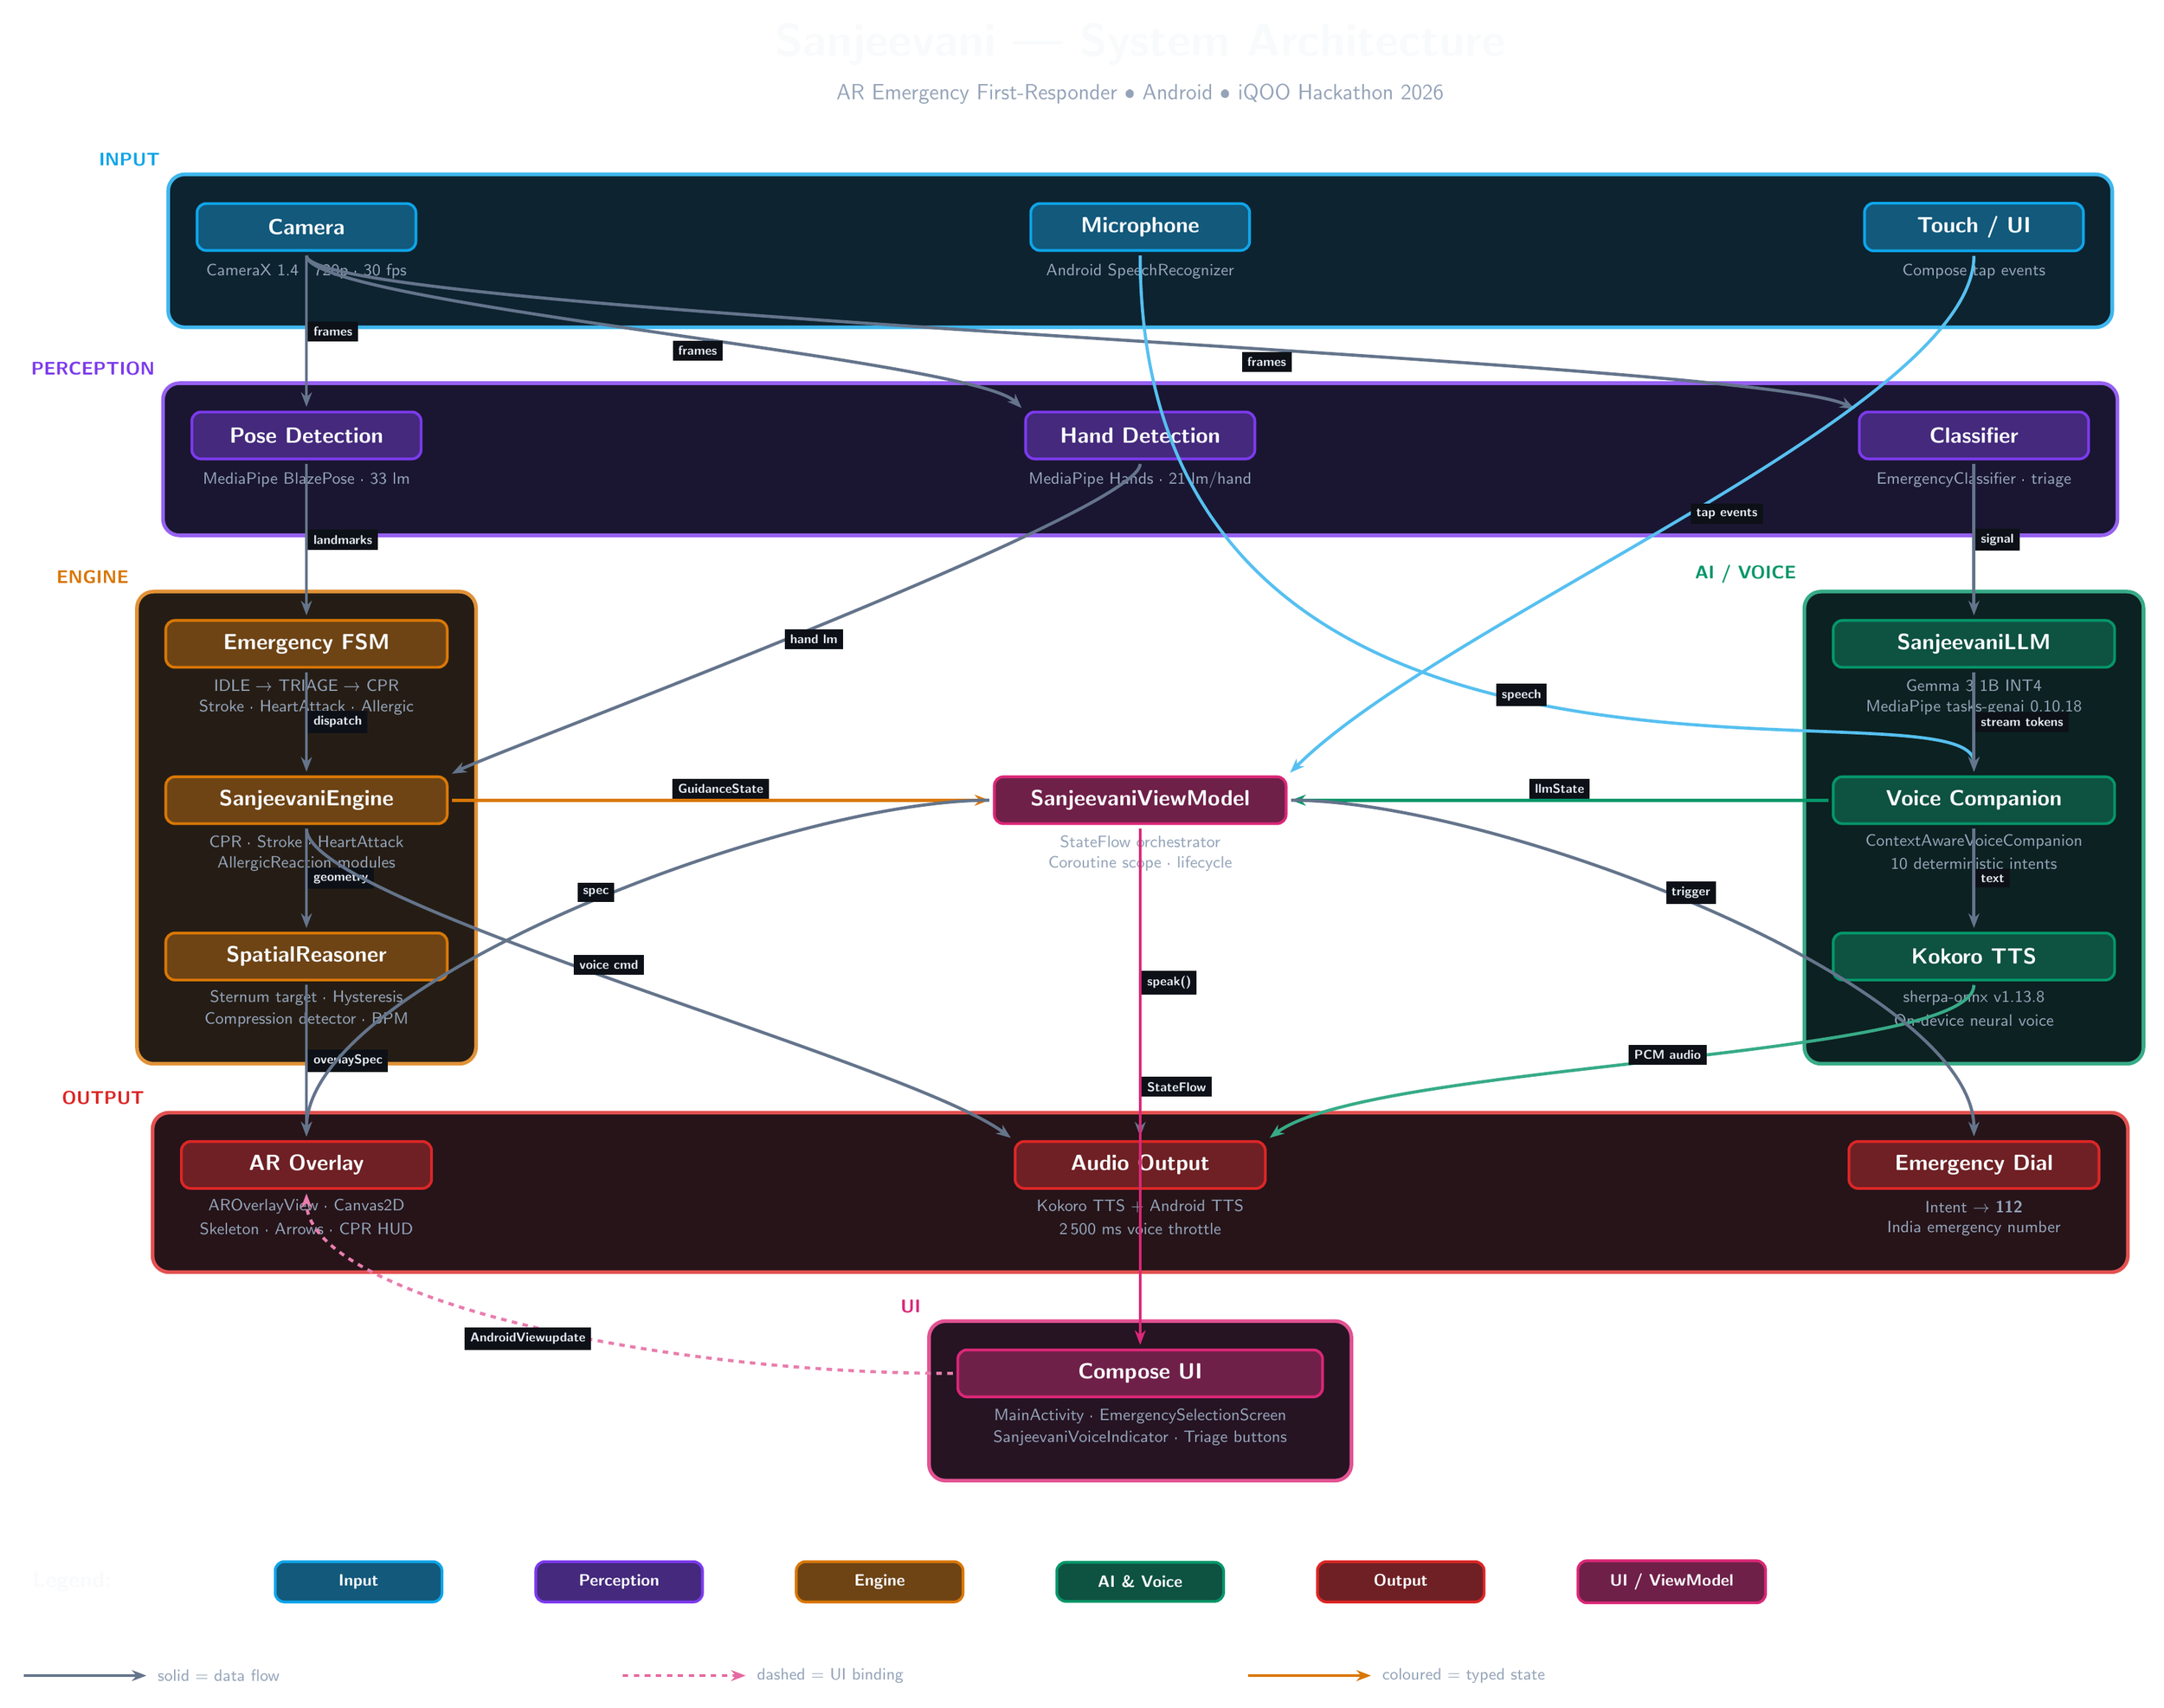
\begin{tikzpicture}

%% ════════════════════════════════════════════════════════════════════════════
%%  TITLE
%% ════════════════════════════════════════════════════════════════════════════
\node[text=cTxt, font=\sffamily\Huge\bfseries] at (26,34.5) (title)
  {Sanjeevani — System Architecture};
\node[text=cSub, font=\sffamily\large] at (26,33.55)
  {AR Emergency First-Responder \textbullet{} Android \textbullet{} iQOO Hackathon 2026};

%% ════════════════════════════════════════════════════════════════════════════
%%  LAYER 1 – INPUT  (y = 31)
%% ════════════════════════════════════════════════════════════════════════════
\node[nd={cIn}{4.2cm}] at (10,31)  (camera) {Camera};
\node[sl] at (10,30.15)  {CameraX 1.4 · 720p · 30 fps};

\node[nd={cIn}{4.2cm}] at (26,31)  (mic)    {Microphone};
\node[sl] at (26,30.15)  {Android SpeechRecognizer};

\node[nd={cIn}{4.2cm}] at (42,31)  (touch)  {Touch / UI};
\node[sl] at (42,30.15)  {Compose tap events};

\begin{pgfonlayer}{background}
\node[lyr=cIn,
      fit={(camera)(mic)(touch)
           ([yshift=-26pt]camera.south)([yshift=-26pt]touch.south)},
      label={[text=cIn,font=\sffamily\normalsize\bfseries]north west:INPUT}]
  (L1) {};
\end{pgfonlayer}

%% ════════════════════════════════════════════════════════════════════════════
%%  LAYER 2 – PERCEPTION  (y = 27)
%% ════════════════════════════════════════════════════════════════════════════
\node[nd={cPerc}{4.4cm}] at (10,27) (pose)   {Pose Detection};
\node[sl] at (10,26.15)  {MediaPipe BlazePose · 33 lm};

\node[nd={cPerc}{4.4cm}] at (26,27) (hand)   {Hand Detection};
\node[sl] at (26,26.15)  {MediaPipe Hands · 21 lm/hand};

\node[nd={cPerc}{4.4cm}] at (42,27) (classif){Classifier};
\node[sl] at (42,26.15)  {EmergencyClassifier · triage};

\begin{pgfonlayer}{background}
\node[lyr=cPerc,
      fit={(pose)(hand)(classif)
           ([yshift=-26pt]pose.south)([yshift=-26pt]classif.south)},
      label={[text=cPerc,font=\sffamily\normalsize\bfseries]north west:PERCEPTION}]
  (L2) {};
\end{pgfonlayer}

%% ════════════════════════════════════════════════════════════════════════════
%%  LAYER 3A – ENGINE  (left, y = 17–23)
%% ════════════════════════════════════════════════════════════════════════════
\node[nd={cEng}{5.4cm}] at (10,23) (fsm)  {Emergency FSM};
\node[sl] at (10,22.2)  {IDLE → TRIAGE → CPR};
\node[sl] at (10,21.78) {Stroke · HeartAttack · Allergic};

\node[nd={cEng}{5.4cm}] at (10,20) (eng)  {SanjeevaniEngine};
\node[sl] at (10,19.2)  {CPR · Stroke · HeartAttack};
\node[sl] at (10,18.78) {AllergicReaction modules};

\node[nd={cEng}{5.4cm}] at (10,17) (spr)  {SpatialReasoner};
\node[sl] at (10,16.2)  {Sternum target · Hysteresis};
\node[sl] at (10,15.78) {Compression detector · BPM};

\begin{pgfonlayer}{background}
\node[lyr=cEng,
      fit={(fsm)(eng)(spr)([yshift=-30pt]spr.south)},
      label={[text=cEng,font=\sffamily\normalsize\bfseries]north west:ENGINE}]
  (L3A) {};
\end{pgfonlayer}

%% ════════════════════════════════════════════════════════════════════════════
%%  LAYER 3B – AI / VOICE  (right, same y band)
%% ════════════════════════════════════════════════════════════════════════════
\node[nd={cAI}{5.4cm}] at (42,23) (llm)   {SanjeevaniLLM};
\node[sl] at (42,22.2)  {Gemma 3 1B INT4};
\node[sl] at (42,21.78) {MediaPipe tasks-genai 0.10.18};

\node[nd={cAI}{5.4cm}] at (42,20) (vcomp) {Voice Companion};
\node[sl] at (42,19.2)  {ContextAwareVoiceCompanion};
\node[sl] at (42,18.78) {10 deterministic intents};

\node[nd={cAI}{5.4cm}] at (42,17) (tts)   {Kokoro TTS};
\node[sl] at (42,16.2)  {sherpa-onnx v1.13.8};
\node[sl] at (42,15.78) {On-device neural voice};

\begin{pgfonlayer}{background}
\node[lyr=cAI,
      fit={(llm)(vcomp)(tts)([yshift=-30pt]tts.south)},
      label={[text=cAI,font=\sffamily\normalsize\bfseries]north west:AI / VOICE}]
  (L3B) {};
\end{pgfonlayer}

%% ── ViewModel (centre of engine–AI band) ─────────────────────────────────
\node[nd={cUI}{5.6cm}] at (26,20) (vm) {SanjeevaniViewModel};
\node[sl] at (26,19.2)  {StateFlow orchestrator};
\node[sl] at (26,18.78) {Coroutine scope · lifecycle};

%% ════════════════════════════════════════════════════════════════════════════
%%  LAYER 4 – OUTPUT  (y = 13)
%% ════════════════════════════════════════════════════════════════════════════
\node[nd={cOut}{4.8cm}] at (10,13) (ar)    {AR Overlay};
\node[sl] at (10,12.2)  {AROverlayView · Canvas2D};
\node[sl] at (10,11.78) {Skeleton · Arrows · CPR HUD};

\node[nd={cOut}{4.8cm}] at (26,13) (audio) {Audio Output};
\node[sl] at (26,12.2)  {Kokoro TTS + Android TTS};
\node[sl] at (26,11.78) {2\,500 ms voice throttle};

\node[nd={cOut}{4.8cm}] at (42,13) (dial)  {Emergency Dial};
\node[sl] at (42,12.2)  {Intent $\to$ \textbf{112}};
\node[sl] at (42,11.78) {India emergency number};

\begin{pgfonlayer}{background}
\node[lyr=cOut,
      fit={(ar)(audio)(dial)
           ([yshift=-30pt]ar.south)([yshift=-30pt]dial.south)},
      label={[text=cOut,font=\sffamily\normalsize\bfseries]north west:OUTPUT}]
  (L4) {};
\end{pgfonlayer}

%% ════════════════════════════════════════════════════════════════════════════
%%  LAYER 5 – COMPOSE UI  (y = 9)
%% ════════════════════════════════════════════════════════════════════════════
\node[nd={cUI}{7.0cm}] at (26,9)  (compose) {Compose UI};
\node[sl] at (26,8.18)  {MainActivity · EmergencySelectionScreen};
\node[sl] at (26,7.76)  {SanjeevaniVoiceIndicator · Triage buttons};

\begin{pgfonlayer}{background}
\node[lyr=cUI,
      fit={(compose)([yshift=-30pt]compose.south)},
      label={[text=cUI,font=\sffamily\normalsize\bfseries]north west:UI}]
  (L5) {};
\end{pgfonlayer}

%% ════════════════════════════════════════════════════════════════════════════
%%  ARROWS
%% ════════════════════════════════════════════════════════════════════════════

%% ── INPUT → PERCEPTION  (Camera feeds all three) ────────────────────────
\draw[ar] (camera.south) -- node[el,right]{frames} (pose.north);
\draw[ar] (camera.south) .. controls +(0,-1) and +(-1,1) ..
    node[el,below,pos=0.55]{frames} (hand.north west);
\draw[ar] (camera.south) .. controls +(0,-1.2) and +(-2,1) ..
    node[el,below,pos=0.6]{frames} (classif.north west);

%% ── Mic → VoiceCompanion  (speech recognition path) ─────────────────────
\draw[ar,cIn!70] (mic.south) .. controls +(0,-12) and +(0,2) ..
    node[el,right,pos=0.45]{speech} (vcomp.north);

%% ── Touch → ViewModel ────────────────────────────────────────────────────
\draw[ar,cIn!70] (touch.south) .. controls +(0,-3) and +(3,3) ..
    node[el,right,pos=0.5]{tap events} (vm.north east);

%% ── PERCEPTION → ENGINE / AI ─────────────────────────────────────────────
\draw[ar] (pose.south) -- node[el,right]{landmarks} (fsm.north);
\draw[ar] (hand.south) .. controls +(0,-1) and +(1,0.5) ..
    node[el,below,pos=0.5]{hand lm} (eng.north east);
\draw[ar] (classif.south) -- node[el,right]{signal} (llm.north);

%% ── ENGINE internal ──────────────────────────────────────────────────────
\draw[ar] (fsm.south) -- node[el,right]{dispatch} (eng.north);
\draw[ar] (eng.south) -- node[el,right]{geometry} (spr.north);

%% ── AI / VOICE internal ──────────────────────────────────────────────────
\draw[ar] (llm.south)   -- node[el,right]{stream tokens} (vcomp.north);
\draw[ar] (vcomp.south) -- node[el,right]{text} (tts.north);

%% ── ENGINE → ViewModel  (GuidanceState) ─────────────────────────────────
\draw[ar,cEng] (eng.east)   -- node[el,above]{GuidanceState} (vm.west);

%% ── AI → ViewModel  (llmState / isSpeaking) ─────────────────────────────
\draw[ar,cAI]  (vcomp.west) -- node[el,above]{llmState} (vm.east);

%% ── ENGINE → OUTPUT ──────────────────────────────────────────────────────
\draw[ar] (spr.south)  -- node[el,right]{overlaySpec} (ar.north);
\draw[ar] (eng.south)  .. controls +(0,-1.5) and +(-2,1.5) ..
    node[el,right,pos=0.45]{voice cmd} (audio.north west);

%% ── TTS → Audio output ───────────────────────────────────────────────────
\draw[ar,cAI!80] (tts.south) .. controls +(0,-1.5) and +(2,1.5) ..
    node[el,left,pos=0.45]{PCM audio} (audio.north east);

%% ── ViewModel → Emergency Dial ───────────────────────────────────────────
\draw[ar] (vm.east) .. controls +(4,0) and +(0,3) ..
    node[el,right,pos=0.45]{trigger} (dial.north);

%% ── ViewModel → Output (AR spec binding) ────────────────────────────────
\draw[ar] (vm.west) .. controls +(-4,0) and +(0,3) ..
    node[el,left,pos=0.45]{spec} (ar.north);

%% ── ViewModel → Audio (isSpeaking / speak()) ─────────────────────────────
\draw[ar] (vm.south) -- node[el,right]{speak()} (audio.north);

%% ── ViewModel → Compose (StateFlow) ─────────────────────────────────────
\draw[ar,cUI] (vm.south) .. controls +(0,-2) and +(0,2) ..
    node[el,right]{StateFlow} (compose.north);

%% ── Compose → AR Overlay (AndroidView binding, dashed) ──────────────────
\draw[ard,cUI!60] (compose.west) .. controls +(-6,0) and +(0,-2) ..
    node[el,left,pos=0.4]{AndroidView\\update} (ar.south);

%% ════════════════════════════════════════════════════════════════════════════
%%  LEGEND
%% ════════════════════════════════════════════════════════════════════════════
\node[text=cTxt,font=\sffamily\large\bfseries] at (5.5,5.0) (leg0) {Legend:};

\node[nd={cIn}{3.2cm},   minimum height=0.75cm, font=\sffamily\small\bfseries]
    at (11,5.0) {Input};
\node[nd={cPerc}{3.2cm}, minimum height=0.75cm, font=\sffamily\small\bfseries]
    at (16,5.0) {Perception};
\node[nd={cEng}{3.2cm},  minimum height=0.75cm, font=\sffamily\small\bfseries]
    at (21,5.0) {Engine};
\node[nd={cAI}{3.2cm},   minimum height=0.75cm, font=\sffamily\small\bfseries]
    at (26,5.0) {AI \& Voice};
\node[nd={cOut}{3.2cm},  minimum height=0.75cm, font=\sffamily\small\bfseries]
    at (31,5.0) {Output};
\node[nd={cUI}{3.6cm},   minimum height=0.75cm, font=\sffamily\small\bfseries]
    at (36.2,5.0) {UI / ViewModel};

%% Arrow types
\draw[ar]  (4.5,3.2) -- +(2.5,0)
    node[right,text=cSub,font=\sffamily\small]{solid = data flow};
\draw[ard,cUI!70] (16,3.2) -- +(2.5,0)
    node[right,text=cSub,font=\sffamily\small]{dashed = UI binding};
\draw[ar,cEng] (28,3.2) -- +(2.5,0)
    node[right,text=cSub,font=\sffamily\small]{coloured = typed state};

\end{tikzpicture}
\end{document}
